
\documentclass{article}

\usepackage{mhchem} % Package for chemical equation typesetting
\usepackage{siunitx} % Provides the \SI{}{} command for typesetting SI units

\usepackage{graphicx} % Required for the inclusion of images
\usepackage[utf8]{inputenc}
\usepackage{CJK}
\usepackage{float}
\usepackage[T1]{fontenc}     %>的正常输出

%\setlength\parindent{2pt} % Removes all indentation from paragraphs
\usepackage{indentfirst} 
\setlength{\parindent}{2em}

\renewcommand{\labelenumi}{\alph{enumi}.} % Make numbering in the enumerate environment by letter rather than number (e.g. section 6)
\newcommand{\tabincell}[2]
{
	\begin{tabular}
	{@{}#1@{}}#2
	\end{tabular}
}

%\usepackage{times} % Uncomment to use the Times New Roman font

%----------------------------------------------------------------------------------------
%	DOCUMENT INFORMATION
%----------------------------------------------------------------------------------------

\title{Postgresql存储管理中的哈希} % Title

\author{马文韬} % Author name

\date{\today} % Date for the report

\begin{document}
\begin{CJK*}{UTF8}{gkai}

\maketitle % Insert the title, author and date

\section{概述}
\subsection{引言}
\indent 众所周知,哈希在计算机程序设计及各种软件系统实现中作用巨大,值得深入研究和探讨。\\
\indent 这篇总结主要讲述我在对Postgresql数据库中存储管理部分的哈希桶和哈希表的使用进行分析研究时候的心得体会,尽量阐述清楚这一部分的相关内容,如有纰漏欢迎指出。
\subsection{存储管理中的哈希}
\begin{figure}[H]
\centering
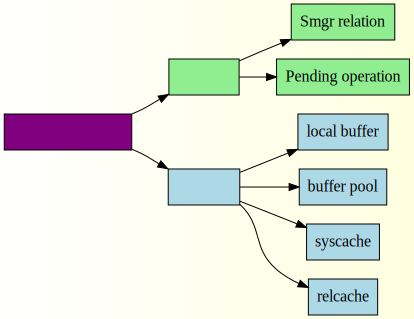
\includegraphics[width = 0.8\textwidth]{index.jpg}
\caption{存储管理中的哈希图}
\label{overflow}
\end{figure}
\indent 如Figure-1,存储管理分为内存(包括缓存)和外存,内存外存各部分又包括几个子模块。在相关的模块中,比如SysCache,SMGR等,哈希表或者哈希桶都得到了广泛的应用,而且作用非常重要。本文就对上图所示的几个相关部分进行研究和阐述。










\section{Hash table基本结构及其操作} 
\subsection{哈希表的基本概念}
\indent 哈希表(Hash table,也叫紧凑表),是根据关键字(Key value)而直接查询在內存存储位置的资料结构。也就是说,它通过把键值通过一个函数的计算,映射到表中一个位置來查询记录,这加快了查找速度。这个映射函数称作哈希函数,存放记录的数组称作哈希表。

\indent 一个通俗的例子是,为了查找电话簿中某人的号码,可以创建一个按照人名首字母顺序排列的表(即建立人名x到首字母F(x)的一個函数关系),在首字母为W的表中查找「王」姓的电话号码,显然比直接查找就要快得多。这里使用人名作为关键字,「取首字母」是这个例子中哈希函数的函数法则F(),存放首字母的表对应哈希表。关键字和函数法则理论上可以任意确定。
\subsection{pg中的哈希表基本结构和相关函数}
\subsubsection{hash table}
\begin{figure}[H]
\begin{center}
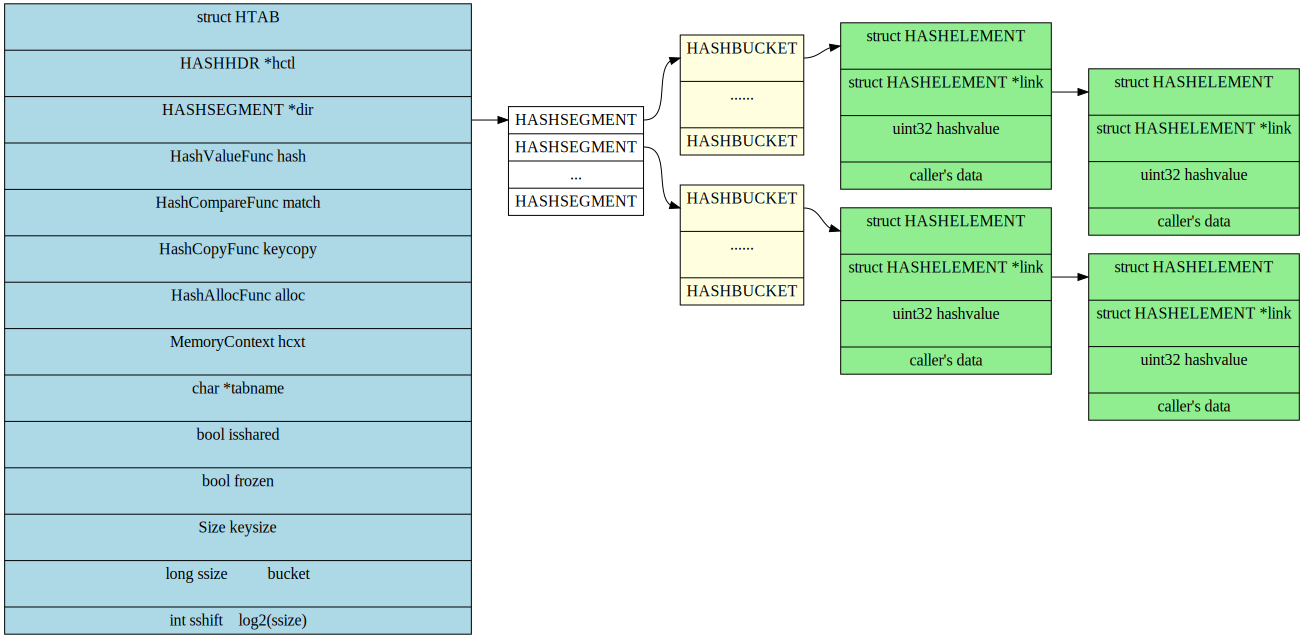
\includegraphics[width=1.0\textwidth]{hash.jpg}
\caption{hash table 结构图}
\end{center}
\end{figure}

\indent 如图Figure-2,hash table的结构图,由图中可以窥探到一个哈希表的基本结构:段指针指向段空间,其中包含多个段,每个段空间内部有多个哈希桶,每个桶指向一个哈希entry链表。对于每一个哈希entry,私有部分为指向下一个entry的指针,还有就是32位的hashvalue域,具体存储的数据由HASHHDR结构体的相关字段来指定大小,再根据偏移量获取和存储数据。

\subsubsection{HASHHDR结构体}
\begin{figure}[H]
	\centering
	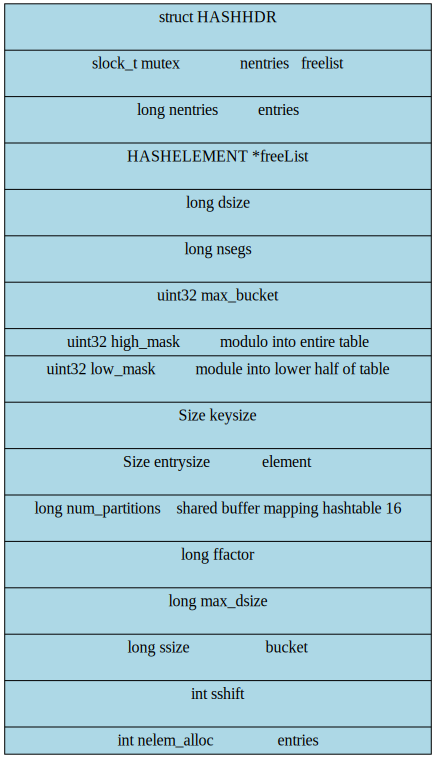
\includegraphics[width=0.6\textwidth]{hashhdr.jpg}
	\caption{HASHHDR结构体}
\end{figure}
\indent HASHHDR结构体用于“contains all changeable info”,在哈希表的初始化阶段和改变的时候都要用到这个结构体,通过对相关参数进行设置修改来决定哈希表的大小等参数。
\indent 如果哈希表是共享内存的哈希表,那么HASHHDR结构体需要保存在共享内存中。对于非共享内存的哈希表而言,\\HASHHDR和HTAB在功能上是相同的。
\subsubsection{哈希结构体中的函数指针}

\begin{table}[H]
\centering
\caption{哈希结构体中函数指针的默认函数及其功能}
\label{address}
\begin{tabular}{|c|c|}
\hline
函数指针  &  相关函数 \\
\hline
HashValueFunc hash & 
\tabincell{c}{ string\_hash 计算string哈希值\\tag\_hash 计算tag哈希值\\oid\_hash 计算oid的哈希值\\bitmap\_hash计算bitmap哈希}\\
\hline
HashCompareFunc match & \tabincell{c}{ string\_compare,如果不自定义,默认\\bitmap\_match 和bitmap\_hash一起用}\\
\hline
HashCopyFunc keycopy & \tabincell {c}{strlcpy 可以自定义,默认}\\
\hline
HashAllocFunc alloc  & \tabincell{c}{DynaHashAlloc  调用上下文\\中定义的内存分配方法}\\
\hline
\end{tabular}
\end{table}

\indent 由Table 1可以看到相关指针函数,这些函数在对哈希表进行创建、查找、添加、删除等操作的时候会被提前设置,如果没有设置的话会调用系统或者上下文默认的函数来执行。


\subsubsection{重要函数}
\indent 在pg中哈希表的实现里,hash\_起着至关重要的作用,完成了包括插入、删除、查找等一系列动作。在整个pg存储部分中这个函数也是使用最频繁的。
\indent hash\_search的函数定义如下:\\

\indent \textbf{ void *hash\_search(HTAB *hashp,   void *keyPtr,   HASHACTION action,   bool *foundPtr);}\\

\indent \textbf{相关参数:}
\begin{itemize}
	\item HTAB *hashp {}哈希表的指针,指向要操作的哈希表
	\item void *keyPtr {}键指针,指向键值
	\item HASHACTION action {}这个函数的action
	\item bool foundPtr {}用引用来指明函数是否找到相关entry,找到了返回true,否则为false,也可以设置为NULL。
\end{itemize}

\textbf{action类型:}
\begin{table}[H] 
\centering
\caption{hash\_search相关操作action标记}
\begin{tabular}{|c|c|c|}
\hline
 HASH\_FIND & \tabincell{c}{ 根据key\\查找哈希表} \\
\hline
 HASH\_ENTER & \tabincell{c}{ 查找哈希表,\\如果entry没出现,\\那么创建一个 }\\
\hline
 HASH\_ENTER\_NULL & \tabincell{c}{查找哈希表,\\如果超出内存,\\返回NULL}  \\
\hline
 HASH\_REMOVE &\tabincell{c} {移除有特定key的entry} \\
\hline
\end{tabular}
\end{table}

\indent 根据上表,action基本类型和作用都在里面,通过指定相关类型和参数来完成各种哈希操作。

\subsection{本章总结}
\indent 本章讲解了pg中哈希表的基本构成和相关的操作函数、重要的结构体等内容,整个存储管理的哈希表都是这个结构。这里明确一下这个结构和相关功能,方便下面具体介绍各个部分的哈希表的使用。\\
\indent 本章主要涉及的c语言源文件 backend/utils/hash目录下的文件及其头文件。








\section{Smgr relation中的Hash} 
\subsection{SMGR功能简介}
\indent 外存管理负责处理数据库与外存介质(在PostgreSQL中只实现了磁盘管理的操作)的交互过程。在pg中,外存管理由SMGR(代码在smgr.c)提供对外操作的统一接口。SMGR负责统管各种介质的管理器,根据上层的请求选择一个具体的介质管理器进行操作。


\subsection{SMGR中哈希表相关的数据结构}
\indent SMGR中哈希表相关的查询、插入、删除等操作都是以RelFileNode结构体作为键来执行的。\\
RelFileNode结构体字段:
\begin{itemize}
\item \quad Oid spcNode:表空间
\item \quad Oid dbNode :数据库
\item \quad Oid relNode:关系
\end{itemize}
\indent RelFileNode结构体保存了表空间、数据库和相关关系的Oid字段。


\begin{figure}[H]
\centering
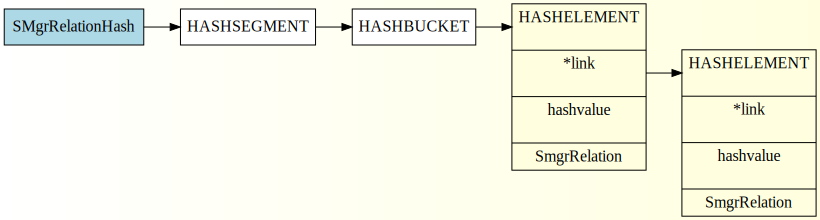
\includegraphics[width = \textwidth]{smgr.jpg}
\caption{smgr中的哈希}
\label{overflow}
\end{figure}

\indent 由上图不难看出,SMGR hash table基本结构和之前讲到的hash table是一样的,在这里表的名称是SMgrRelationHash,每一个entry中的数据除了私有部分,还保存着SMgrRelation,也就是SMGR关系。SMGR部分的哈希操作主要就是对SMgrRelation关系的查询、插入等等。

\subsection{SMGR中哈希函数的相关调用}
\indent 在SMGR中有几处都使用了hash\_search函数,如下表所示:

\begin{table}[H] 
\centering
\scriptsize
\caption{smgr relation中的哈希函数}
\begin{tabular}{|c|c|c|c|}
\hline
\tabincell{c}{函数名}  &
\tabincell{c}{参数}  &
\tabincell{c}{调用函数} &
\tabincell{c}{使用场景}\\
\hline
\tabincell{c}{hash\_search}&
\tabincell{c}{SMgrRelationHash,\\(void *)\&rnode,\\HASH\_ENTER,\\\&found}&
\tabincell{c}{SMgrRelation  \\smgropen\\(RelFileNode rnode)}&
\tabincell{c}{RelFileNode作为键\\查找并返回SMgrRelation对象,\\找不到就创建一个}\\
\hline
\tabincell{c}{hash\_search}&
\tabincell{c}{SMgrRelationHash,\\\&(reln->smgr\_rnode),\\HASH\_REMOVE,\\NULL}&
\tabincell{c}{void \\smgrclose\\(SMgrRelation reln)}&
\tabincell{c}{smgr关系的RelFileNode\\作主键查找并删除\\SMgrRelation对象}\\
\hline
\tabincell{c}{hash\_search}&
\tabincell{c}{SMgrRelationHash,\\(void *)\&rnode\\HASH\_FIND,\\NULL}&
\tabincell{c}{ void \\smgrclosenode\\(RelFileNode rnode)}&
\tabincell{c}{RelFileNode作为键查找返回\\相应SMgrRelation对象,\\由smgrclose完成删除\\避免创建无用关系}\\
\hline
\end{tabular}
\end{table}

\indent 在表中的函数中,hash\_search指定的action为HASH\_ENTER、\\HASH\_REMOVE以及HASH\_FIND,这些函数将以RelFileNode作为键对\\SMgrRelationHash这个哈希表进行插入、删除和查找SMgrRelation的操作。

\subsection{本章小结}  
\indent 本章主要对SMGR管理部分的哈希函数及哈希表的使用进行简单的介绍。相关代码主要在backend/storage/smgr/smgr.c中。


\section{Pending operation中的Hash} 

\subsection{Pending operation哈希表功能简介}
\indent Pending operation哈希表的主要用途是记录同步磁盘的操作,添加或者删除相关的同步操作。\\
\subsection{Pending operation哈希表及相关结构}
\indent PendingOperationTag结构体是对哈希表查询的键,其字段如下:

\begin{itemize}
\item \quad RelFileNode rnode;
\item \quad ForkNumber forkNum;
\item \quad BlockNumber  segno;
\end{itemize}

\indent Pending operation哈希表的基本结构如下图:

\begin{figure}[H] 
\centering
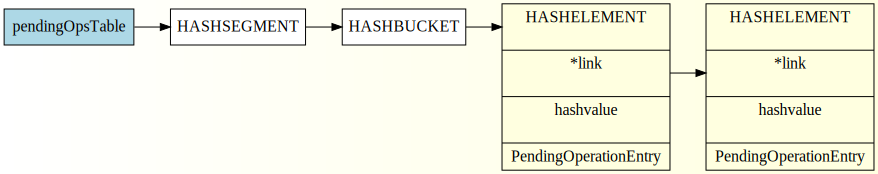
\includegraphics[width = \textwidth]{pending.jpg}
\caption{pending operation中的哈希}
\label{overflow}
\end{figure}
\indent pendingOpsTable是哈希表的名称,entry存储的数据是PendingOperationEntry结构体,其字段如下:
\begin{itemize}
\item \quad PendingOperationTag:作为key。
\item \quad bool canceled:标志位,表示相关操作是否已经被取消。
\item \quad CycleCtr cycle\_ctr;
\end{itemize}

\subsection{Pending operation的哈希函数调用}
\indent Pending operation中哈希函数的相关调用如下表:
\begin{table}[H] 
\scriptsize
\centering

\caption{pending operation中的哈希函数}
\begin{tabular}{|c|c|c|c|}

\hline
\tabincell{c}{函数名}  &
\tabincell{c}{参数}  &
\tabincell{c}{调用函数} &
\tabincell{c}{使用场景}\\
\hline
\tabincell{c}{hash\_search}&
\tabincell{c}{pendingOpsTable,\\\&entry->tag,\\HASH\_REMOVE,\\NULL}&
\tabincell{c}{void mdsync(void)}&
\tabincell{c}{写操作同步到磁盘时\\删除已经无效的操作\\,PendingOperationTag\\作为键查找相应操作并移除}\\
\hline
\tabincell{c}{hash\_search}&
\tabincell{c}{pendingOpsTable,\\\&key,HASH\_ENTER,\\\&found}&
\tabincell{c}{void RememberFsyncRequest\\(RelFileNode rnode,\\ForkNumber forknum,\\BlockNumber segno)}&
\tabincell{c}{PendingOperationTag作为\\主键将fsync的请求\\添加到哈希表中}\\
\hline
\end{tabular}
\end{table}

\indent 由表可见,这部分的主要操作是两个,一个是将新来的同步请求添加到pendingOpsTable哈希表中,另外就是将取消的或者已经完成的同步操作移除出哈希表。

\subsection{本章小结}
\indent 本章主要对Pending Operation部分的哈希操作进行介绍,相关代码主要在backend/storage/md.c中。










\section{SysCache中的Hash} 
\subsection{SysCache简介}
\indent SysCache主要用于缓存系统表元组。PostgreSQl8.4.1版本有54个系统表。每个系统表用一个CatCache结构体来保存相关数据。在结构体内部使用Hash来存储被缓存的系统表元组。每个CatCache有小于等于四个关键字,可以利用这些关键字的多个或者全部来查找相关元组。

\subsection{SysCache中哈希的相关结构}

\indent SysCache整个结构的示意图如下:
\begin{figure}[H] 
\centering
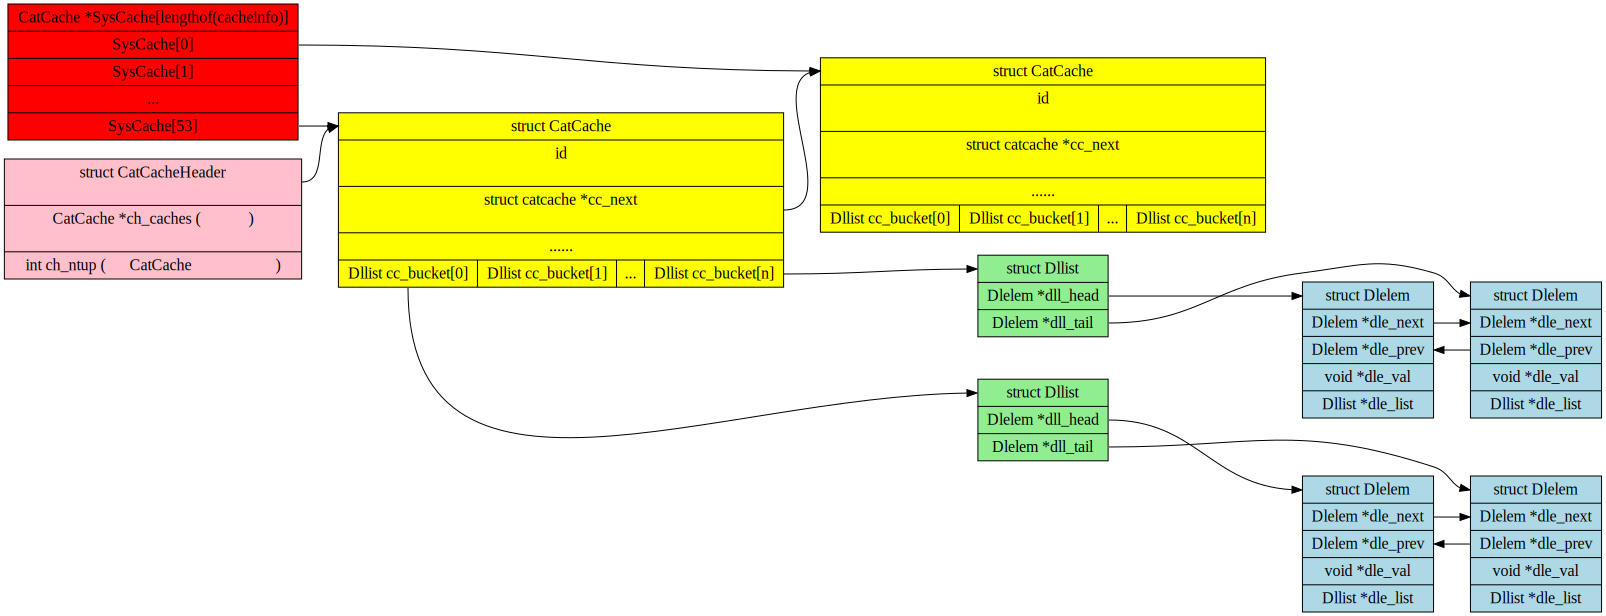
\includegraphics[width = \textwidth]{syscache.jpg}
\caption{hash桶结构图}
\label{overflow}
\end{figure}
\indent 如图所示,每个CatCache包含若干个哈希桶,哈希桶内部由Dlelem组成双链表,由Dllist指向该链表。Dlelem中保存相应的系统表元组信息。查询也就是针对相应CatCache表中的元组信息进行。\\

\indent CatCache的结构如下图,其中哈希相关的字段记录了哈希键个数、哈希桶的指针以及存储键的数组。
\begin{figure}[H] 
\centering
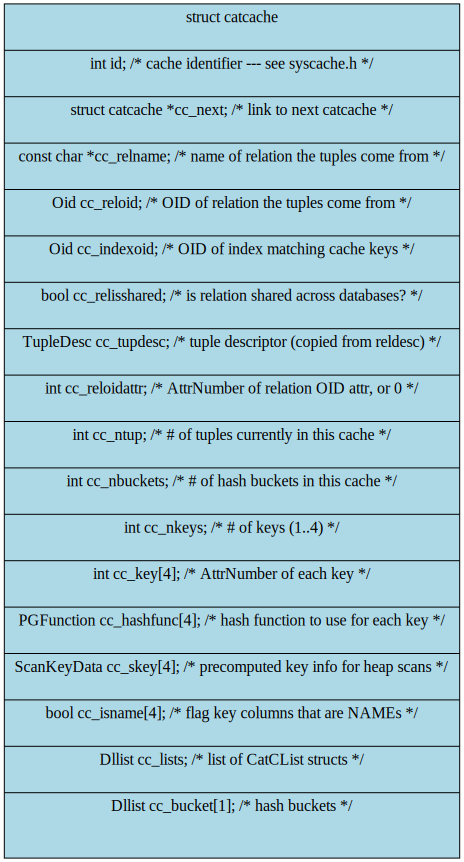
\includegraphics[width = 0.4\textwidth]{catcache.jpg}
\caption{CatCache结构图}
\label{overflow}
\end{figure}


\subsection{SysCache中的相关查询操作}
\indent SysCache中的查询操作有两种:精确匹配和部分匹配。
\subsubsection{精确匹配}

\begin{enumerate}
	\item 初始化关键字信息,根据四个键值初始化cur\_skey键值数组,\\CatalogCacheComputeHashValue函数根据四个键值计算hashValue,\\HASH\_INDEX宏利用hashValue和cc\_buckets计算索引。
	\item 查找,HeapKeyTest匹配键值,在Hash桶中找到满足的Dlelem,\\将该Dlelem移动到链表头部,方便下次访问。
	\item 如果没找到,则对物理系统表进行扫描,确定相应元组是否真的是不存在或者仅仅是没在缓存中。如果找到了,就将相应元组加到链表头部,否则构建一个只有键值的“负元组”,放到桶内部链表头部。
\end{enumerate}


\subsubsection{部分匹配}
\begin{enumerate}

	\item 初始化关键字信息,根据部分关键字初始化cur\_skey。
	\item 计算哈希值和索引,CatalogCacheComputeHashValue根据关键字个数计算lhashValue。
	\item 在CatCache的cc\_lists\\指向的CatCList链表中查找,HeapKeyTest检查key是否匹配,将匹配的CatClist放到cc\_lists链表的头部,不存在CatCList,扫描物理表并构建。\\
\end{enumerate}

\subsection{本章小结}
\indent 本章介绍了SysCache中相关的哈希操作,SysCache不同于之前的是它利用的是哈希桶,而不是之前的几个模块用到的哈希表。这部分的相关代码主要在backend/utils/cache/syscache.c,catcache.c中。



\section{RelCache中的Hash} 

\subsection{RelCache简介}
\indent RelCache用于缓存关系元组,因为大多数RelationData是不变的,所以pg仅用一个哈希表来维护这个结构。
\subsection{RelCache中哈希表结构}

\indent Relation 的Oid作为key进行查询。\\
\indent Relache中哈希表的结构如图:

\begin{figure}[H] 
\centering
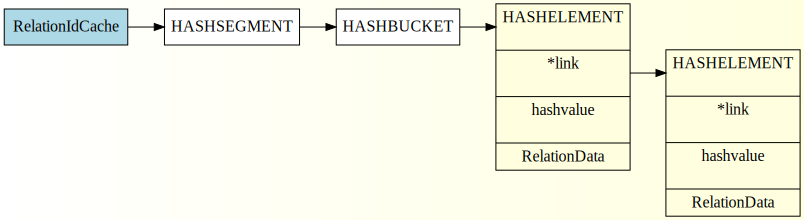
\includegraphics[width = \textwidth]{rel.jpg}
\caption{RelCache中的哈希}
\label{overflow}
\end{figure}

\indent   如图所示,哈希表的名称是RelationIdCache,entry中存储的数据是RelationData结构体。对哈希表的操作主要就是对这个结构体的写改删查操作。


\subsection{RelCache中哈希函数的使用}

\begin{table}[H] 
\centering

\caption{RelCache中的hash}
\begin{tabular}{|c|c|c|c|}
\hline
\tabincell{c}{函数名}  &
\tabincell{c}{参数}  &
\tabincell{c}{调用宏} &
\tabincell{c}{使用场景}\\
\hline
\tabincell{c}{hash\_search}&
\tabincell{c}{RelationIdCache,\\\&(RELATION->rd\_id),\\HASH\_ENTER\\,\&found}  &
\tabincell{c}{RelationCacheInsert\\(RELATION)} &
\tabincell{c}{以关系的Oid作为\\主键将新的关系\\插入到relcache\\哈希表中}\\
\hline
\tabincell{c}{hash\_search}&
\tabincell{c}{RelationIdCache,\\\&(ID),HASH\_FIND,\\NULL}  &
\tabincell{c}{RelationIdCacheLookup\\(ID,RELATION)}&
\tabincell{c}{用关系Oid作为主键\\在relcache中查找相应对象}\\
\hline
\tabincell{c}{hash\_search}&
\tabincell{c}{RelationIdCache,\\\&(RELATION->rd\_id),\\HASH\_REMOVE,\\NULL}&
\tabincell{c}{RelationCacheDelete\\(RELATION)}&
\tabincell{c}{用关系Oid作为\\主键查找并删除\\relcache相应对象}\\
\hline
\end{tabular}
\end{table}

\indent 由图可知,对哈希的操作主要是根据Oid将相关关系添加或者从表中删除。

\subsection{本章小结}
\indent RelCache相关代码在backend/utils/cache/relcache.c中。






\section{Buffer pool中的Hash} 

\subsection{Buffer pool简介}
\indent 如果需要访问的系统表元组在Cache中无法找到或者需要访问普通表的元组,就需要对缓冲池进行访问。任何对于表、元组、索引表等的操作都在缓冲池中进行。

\subsection{Buffer pool中哈希的相关结构}
\indent Buffer pool的哈希操作用BufferTag作为键,BufferTag的字段:

\begin{itemize}
\item \quad rnode(表空间OID,数据库OID和表OID组成);\\
\item \quad forkNum 枚举类型,标记缓冲区中文件块类型;\\
\item \quad blockNum  块号;
\end{itemize}


\indent buffer pool哈希表结构图如下:
\begin{figure}[H] 
\centering
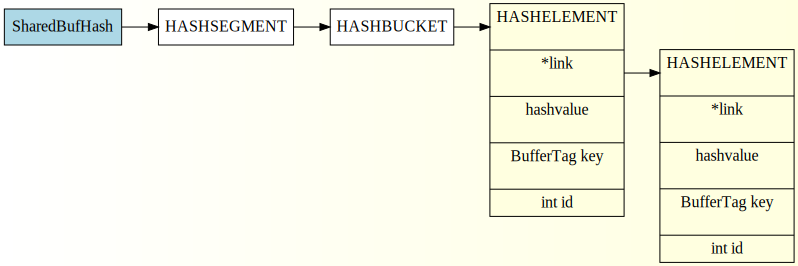
\includegraphics[width = \textwidth]{buf.jpg}
\caption{}
\label{overflow}
\end{figure}
\indent 由图可知,buffer pool中哈希表的名称为SharedBufHash,entry存储的数据有BufferTag和buffer id。

\subsection{Buffer pool中的哈希操作}

\indent Buffer pool中主要的哈希操作如下表:

\begin{table}[H] 
\centering
\scriptsize
\caption{buffer pool中的hash}
\begin{tabular}{|c|c|c|c|}
\hline
\tabincell{c}{函数名}  &
\tabincell{c}{参数}  &
\tabincell{c}{调用函数} &
\tabincell{c}{使用场景}\\
\hline
\tabincell{c}{hash\_search\_with\\\_hash\_value}&
\tabincell{c}{SharedBufHash,\\tagPtr,\\hashcode,\\HASH\_FIND,\\NULL}&
\tabincell{c}{int BufTableLookup\\(BufferTag *tagPtr,\\uint32 hashcode)} &
\tabincell{c}{根据BufferTag\\在SharedBufHash中查询,\\返回buffer ID}\\
\hline
\tabincell{c}{hash\_search\_with\\\_hash\_value}&
\tabincell{c}{SharedBufHash,\\tagPtr,\\hashcode,\\HASH\_REMOVE,\\NULL}&
\tabincell{c}{void BufTableDelete\\(BufferTag *tagPtr,uint32 hashcode)}&
\tabincell{c}{根据BufferTag删除\\SharedBufHash中的entry}\\
\hline
\tabincell{c}{hash\_search\_with\\\_hash\_value}&
\tabincell{c}{SharedBufHash,\\tagPtr,\\hashcode,\\HASH\_ENTER,\\\&found}&
\tabincell{c}{int BufTableInsert(BufferTag *tagPtr,\\uint32 hashcode,\\int buf\_id}&
\tabincell{c}{根据BufferTag和\\buffer ID插入entry,\\如果有冲突entry,\\返回冲突entry的buffer ID}\\
\hline
\end{tabular}
\end{table}

\indent 由上表可知,hash\_search\_with\_hash\_value根据BufferTag添加、查找或删除相关的entry,并返回相应entry的buffer id。

\subsection{本章小结}
\indent 本章主要总结了hash在buffer pool的应用,相关代码在 backend/storage/buffer/buf\_tab.c中。


\section{Local buffer中的Hash} 
\subsection{Local buffer简介}
\indent 本地缓冲池是每个进程特有的,在进程初始化时候创建。本地缓冲池对其它进程不可见。

\subsection{Local buffer哈希表相关结构}
\indent Local buffer的哈希操作用BufferTag作为键,BufferTag的字段:

\begin{itemize}
\item \quad rnode(表空间OID,数据库OID和表OID组成);\\
\item \quad forkNum 枚举类型,标记缓冲区中文件块类型;\\
\item \quad blockNum  块号;
\end{itemize}

\indent Local buffer哈希表结构图如下:

\begin{figure}[H] 
\centering
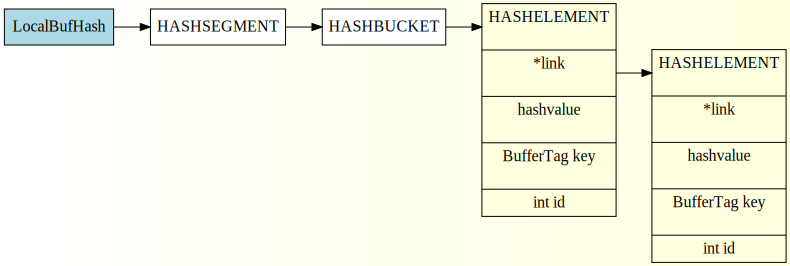
\includegraphics[width = \textwidth]{local.jpg}
\caption{local buffer中的哈希}
\label{overflow}
\end{figure}

\indent 由上图可知,local buffer的哈希表名为LocalBufHash,entry中存储BufferTag和buffer id等内容。

\subsection{Local buffer中的哈希操作}
\indent Local buffer中的哈希操作如下表:
\begin{table}[H] 
\scriptsize

\centering
\caption{local buffer中的哈希函数}
\begin{tabular}{|c|c|c|c|}
\hline
\tabincell{c}{函数名}  &
\tabincell{c}{参数}  &
\tabincell{c}{调用函数} &
\tabincell{c}{使用场景}\\
\hline
\tabincell{c}{hash\_search}&
\tabincell{c}{LocalBufHash,\&newTag,\\HASH\_FIND,NULL}  &
\tabincell{c}{void LocalPrefetchBuffer\\(SMgrRelation smgr,\\ForkNumber forkNum,\\BlockNumber blockNum)} &
\tabincell{c}{异步读取一个关系块\\用smgr等参数创建一个tag,\\查找LocalBufHash中相应块}\\
\hline
\tabincell{c}{hash\_search}&
\tabincell{c}{LocalBufHash,\&newTag,\\HASH\_FIND,NULL}  &
\tabincell{c}{void LocalBufferAlloc\\(SMgrRelation smgr,\\ForkNumber forkNum,\\BlockNumber blockNum,\\bool *foundPtr)} &
\tabincell{c}{用smgr等参数创建一个tag,\\为给定关系的给定页面创建\\local buffer}\\
\hline
\tabincell{c}{hash\_search}&
\tabincell{c}{LocalBufHash,\\\&bufHdr->tag,\\HASH\_REMOVE,NULL}  &
\tabincell{c}{void LocalBufferAlloc\\(SMgrRelation smgr,\\ForkNumber forkNum,\\BlockNumber blockNum,\\bool *foundPtr)} &
\tabincell{c}{更新LocalBufHash,\\移除旧的entry}\\
\hline
\tabincell{c}{hash\_search}&
\tabincell{c}{LocalBufHash,\\\&bufHdr->tag,\\HASH\_ENTER,NULL}  &
\tabincell{c}{void LocalBufferAlloc\\(SMgrRelation smgr,\\ForkNumber forkNum,\\BlockNumber blockNum,\\bool *foundPtr)} &
\tabincell{c}{更新LocalBufHash,\\创建新的entry}\\
\hline
\end{tabular}
\end{table}

\indent 由表可知,BufferTag由调用函数的smgr等参数生成,并用这个BufferTag作为参数对LocalBufHash进行查询,对相应的entry进行写改删查的操作。

\subsection{本章小结}
\indent 本章对Local buffer部分的哈希结构及相关使用进行了提炼和总结,相关函数在backend/storage/buffer/localbuf.c中。

\section{总结}
\indent 众所周知,哈希在计算机程序设计及各种软件系统实现中作用巨大,值得深入研究和探讨。\\
\indent 这篇总结主要讲述作者在对Postgresql数据库中存储管理部分的哈希桶和哈希表的使用进行分析研究时候的心得体会。哈希表和哈希桶的使用相比链表和数组等结构,利用计算来节省查询时间,并且在空间分配和管理等方面都有出色的表现,是一个非常值得学习研究的数据结构。\\
\indent 感谢老师同学尤其是吴军学长在学习过程中对我的帮助!



\end{CJK*}
\end{document}





